%\index{\footnote{}}
\chapter{Introduction}
Developing a unified architectural pipeline for multiclass abnormality classification and grounded localization
in 3D Computed Tomography (CT) addresses two of the most critical imperatives in clinical AI adoption: diagnostic accuracy and explainability.
Specifically, utilizing dense pixellevel segmentation as the mechanism for localization forces the architecture to
provide voxellevel visual evidence for its diagnostic claims. This ensures that the model is held accountable and its
reasoning aligns with clinical diagnosis.

\section{Background}
The transition from 2D projectional radiography to volumetric CT represents a paradigm shift in medical image analysis.
\begin{figure}[H]
\centering

\includegraphics[width=0.8\linewidth]{\detokenize{Chapters/chapter1PIC/2D to 3D.jpg}}
\caption{Transition from 2D projectional radiography to volumetric CT.}
\label{fig:2dto3d}
\end{figure}
For Lung disease diagnosis, Chest Xrays (CXR) are commonly used as the first imaging test due to its low cost and low
radiation exposure. However, studies show that their capability to detect abnormailities is limited when compared to 3D CT.
\cite{SELF2013401}.

Furthermore, CXR has historically benefited from the availability of massive, radiologistannotated datasets, while
the analysis of chest CT volumes has been severely constrained by a lack of such data.
However, the recent introduction of largescale, textpaired datasets has facilitated the development of stateoftheart

(SotA) visionlanguage foundation models tailored specifically for volumetric imaging \cite{baharoon2025rexgroundingct3dchestct,flores2016,chen2026dflashblockdiffusionflash}.


Beyond deep learning approaches, Dictionary Learning algorithms, particularly, Label Consistent KSVD (LCKSVD) \cite{jiang2013lcksvd},
Label Embedded Dictionary Learning (LEDL) and Fischer Discriminant Dictionary Learning (FDDL)
offer viable approaches for interpretable CT analysis. All three techniques incorporate label information during the dictionary training
process, and ensures that the sparse representation of the data is highly discriminative, making them
wellsuited for multiabnormality tasks.

\section{Problem Statement}
The clinical utility of Deep Learningbased approaches is hindered by a lack of interpretability. While tools like GradCAM
provide posthoc explanations to model decisions, these are often insufficient for medical professionals who require a granular
understanding of the model's decision making process. In high stakes environments, a model that produces a diagnosis without
transparency in its reasoning is difficult to integrate into standard workflows, as it lacks the accountability necessary for legal
and ethical compliance.

\begin{figure}[H]
\centering
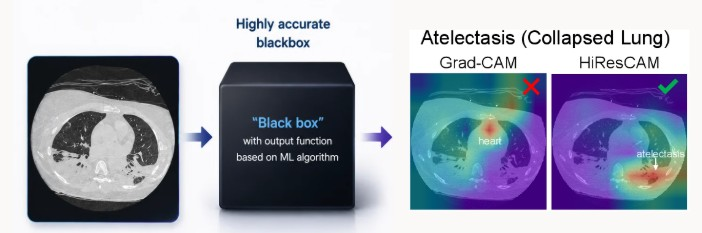
\includegraphics[width=0.8\linewidth]{Chapters/chapter1PIC/HIresCAM.jpg}
\caption{HiResCAM example illustrating higherresolution localization compared with GradCAM.}
\label{fig:hirescam}
\end{figure}

\section{Objectives and Scope}
The primary goal of this project is to address the limitations of existing Deep Learning based approaches for Lung abnormality
classification and localization by developing an inheerntly interpretable dictionary learning framework.
This approach aims to enable transparent, anatomically grounded decision making, where each classification outcome
can be traced back to specific pathological patterns. This aligns with clinical reasoning and facilitates validation and
adoption in radiological workflows. The specific objectives are as follows:

\subsection{Objectives}
\begin{itemize}
	\item Implement a Dictionary Learning approach to learn normal and pathological dictionary atoms using a publicly available annotated 3D chest CT dataset.
	\item Map dictionary atoms back to anatomical features and visualize their spatial contribution maps.
	\item Benchmark model performance against stateoftheart classification and segmentation models on the same dataset.
	\item Evaluate abnormality localization by the model on a realworld dataset with expert radiologist review.
\end{itemize}

\subsection{Scope}
The scope of this study focuses on the development and evaluation of a dictionary learning based approach for classification
and grounded localization of lung abnormalities using volumetric 3D CT data, with the following limitations:

\begin{itemize}
	\item This study is limited to 3 thoracic abnormalities: Pulmonary Nodules, GroundGlass Opacities, and Consolidations, based on expert radiologist recommendation and dataset availbility.
	\item This study will utilize a single publicly available dataset for training and evaluation, which may limit generalizability to other populations and scanner types.
	\item The proposed approach will be limited only to linear methods, and will not explore nonlinear or hybrid models that provide better performance for less explainability.
\end{itemize}

\section{Literature Review}
The landscape of 3D CT analysis is currently divided into three primary architectural paradigms:
\begin{itemize}
	\item Classificationbased models that prioritize diagnostic labels
	\item Segmentationbased models that prioritize boundary precision
	\item Unified architectures designed for grounded localization
\end{itemize}.

SotA models are predominantly specialized in either classification or segmentation. However, recent systems, particularly
in 2025 and 2026, are moving toward multitask learning or foundation models that can perform both diagnosis and voxellevel
segmentation simultaneously.

Table 1 summarizes the key models in each category, their primary task orientation, and their performance on standard benchmarks.

\begin{center}
\captionof{table}{Summary of major 3D CT analysis paradigms and representative models}
\label{tab:3dctparadigms}
\begin{tabularx}{\textwidth}{p{2.8cm} >{\raggedright\arraybackslash}X >{\raggedright\arraybackslash}X >{\raggedright\arraybackslash}X}
\toprule
\textbf{Paradigm} & \textbf{Representative Models} & \textbf{Primary Task} & \textbf{Typical Strengths / Notes} \\
\midrule
Classificationbased & CTCLIP; Merlin; DINOv3 & Imagelevel diagnosis; retrieval; linear probing & Strong imagelevel diagnosis; good zeroshot and transfer performance; efficient inference; limited voxellevel localization. \\
\addlinespace
Segmentationbased & nnUNet; SegVol; SAMMed3D & Voxellevel lesion segmentation & High boundary precision and dense localization; foundation models aim for universal volumetric segmentation across organs and pathologies. \\
\addlinespace
Unified architectures & BiomedParse; MedImageParse; CitrusV; MTMed3D; MedVista3D & Joint diagnosis, segmentation, and reasoning & Multitask inference with grounded localization; integrates report understanding with voxel outputs; typically more complex and computationally intensive. \\
\midrule
\end{tabularx}
\end{center}

\subsection{Classification Architectures}
Classificationbased models for 3D CT have shifted away from 3D Convolutional Neural Networks (CNNs) such as 3D UNet,
3D ResNet and DenseNet pipelines, toward Vision Transformers (ViTs) and selfsupervised encoders. The benchmark for this paradigm is
the CTRATE dataset, which introduced the first public largescale 3D medical imaging dataset with paired textual reports, enabling
the development of Contrastive LanguageImage Pretraining for Computed Tomography (CTCLIP).

CTCLIP is a VLFM designed for 3D chest CT analysis. It extends the CLIP framework to volumetric medical
imaging by jointly learning representations from CT scans and their corresponding radiology reports. \cite{hamamci2024ctclip,radford2021clip}
Through contrastive learning, the model aligns image features with textual descriptions, enabling tasks such as zeroshot classification,
crossmodal retrieval, and reportguided abnormality localization. \cite{hamamci2024ctclip}
The model is particularly effective in learning semantic relationships between radiological findings and volumetric imaging
patterns such as GGO, consolidation, fibrosis, and pulmonary nodules. \cite{hamamci2024ctclip,rexgroundingct}

Recent benchmarks such as Merlin and DINOv3 have further challenged the necessity of domainspecific pretraining.
Merlin is a VLFM exclusively pretrained on abdominal CT scans. Despite it's training, Merlin
has consistently demonstrated exceptional zeroshot performance on chest CT classification tasks, even when it was
restricted to a linear probe, significantly outperforming models like CTCLIP, M3FM, and CTFM that were explicitly
trained on thoracic data, by an average of 12.3\% in Area Under the Receiver Operating Characteristic Curve (AUROC).
Specifically, in crossdomain retrieval tasks, Merlin surpassed CTCLIP by 24.7\%.

DINOv3, a selfsupervised ViT pretrained on over 1.7 billion natural images, outperform specialized medical models like
CTNet and CTCLIP across all metrics on several classification tasks due to it's ability to capture finegrained textural features.

\subsection{Segmentation Architectures}
The prevailing SotA for supervised volumetric segmentation remains variations of the 3D UNet, such as nnUNet, which
utilizes an adaptive framework to optimize preprocessing and architecture for specific datasets. However, the field has
recently shifted toward foundation models capable of universal segmentation such as SegVol and SAMMed3D.
The SegVol model is the first 3D foundation model specifically designed for universal volumetric medical image segmentation.
Similarly, SAMMed3D adapts the Segment Anything Model (SAM) for 3D medical data.

Recent evaluations published at the Machine Learning for Healthcare (MLHC) Conference in 2025, which specifically utilized
the ReXGroundingCT dataset, revealed that the current SotA textprompted segmentation models that demonstrate nearperfect
performance in general computer vision tasks struggle with the nuanced clinical descriptions and illdefined boundaries
of chest CT abnormalities.

\subsection{Unified Architectures}
Recent models have been designed to integrate abnormality detection, segmentation, and multimodal chainofthought reasoning,
enabling pixellevel localization, structured report generation, and physicianlike diagnostic inference in a single framework.
BiomedParse, and it's clouddeployed version MedImageParse, developed by Microsoft, are foundation models designed to parse 3D
medical images.
Other notable models include CitrusV, MTMed3D and MedVista3D, where each architecture incorporates a multitask learning
(MTL) framework~\cite{citrusv2025,mtmed3d2025,medvista3d2025}, as summarized in Table~\ref{tab:3dctparadigms}.

\subsection{Dictionary Learning Approaches}
Applications of sparse dictionary learning in medical imaging have demonstrated significant success across diverse diagnostic tasks. In histopathological
analysis, Discriminative Feature oriented Dictionary Learning (DFDL) has shown the ability to learn class specific dictionaries that achieve high classification
accuracy even with limited training data, a critical advantage when generous training samples are not available~\cite{vu2016dfdl}. In neuroimaging, multi feature kernel supervised
dictionary learning approaches have demonstrated superior performance in distinguishing Alzheimer\'s disease patients from cognitively unimpaired individuals,
achieving 98.18\% classification accuracy while maintaining fast testing times~\cite{li2018mkscddl}.

Most relevant to our work, dictionary learning has been successfully applied to lung disease diagnosis from CT images. One approach utilized both frozen
dictionary learning and label consistent LCKSVD to classify COVID 19 CT scans, achieving 89\% accuracy on the CCCCII dataset~\cite{gould2007nodule}. The framework\'s key
advantage lies in its interpretability, where the sparse coding output can be directly mapped back to the original input signal domain. This work demonstrates that
sparse representation methods offer an effective balance between performance and explainability for lung disease classification tasks, providing clear feature
representations while maintaining competitive accuracy. Similarly, sparse representation methods have achieved 95.4\% accuracy in classifying diffuse lung disease
patterns on HRCT images, effectively handling the high variety and complexity of patterns~\cite{aberle2011nlst}.


\subsection{Explainability Approaches}

GradCAM is one of the most widely used posthoc explanation methods for CNNbased classifiers \cite{selvaraju2017gradcam}. 
It generates classdiscriminative heatmaps by using gradients flowing into the final convolutional layer, allowing the user to identify
image regions that influenced a prediction \cite{selvaraju2017gradcam}. 
It's main limitation is that it produces lowresolution saliency maps and does not directly provide precise lesion boundaries or
voxellevel localization, which is a major drawback for 3D CT interpretation \cite{selvaraju2017gradcam,draelos2021usehirescaminsteadgradcam}.

SegGradCAM extends this idea by adapting GradCAM to semantic segmentation outputs \cite{Suara_2024}. 
Instead of only highlighting regions that are important for imagelevel classification, it produces pixellevel relevance heatmaps for
segmentation predictions \cite{Suara_2024}.
This is particularly useful for volumetric medical imaging tasks where the target abnormality occupies a sparse region within a large 3D scan.

HiResCAM addresses one of the key weaknesses of GradCAM by producing higherresolution and more faithful localization maps \cite{draelos2021usehirescaminsteadgradcam}. 
This is important in chest CT because many abnormalities, such as small nodules, consolidations, or subtle interstitial changes,
may be missed by coarse heatmaps. 
HiResCAM aims to preserve fine spatial detail, making it more suitable for medical imaging applications where precise localization is required \cite{draelos2021usehirescaminsteadgradcam}. 
However, like other gradientbased methods, it remains a posthoc explanation technique and does not change the internal decision process of the model.

\section{Report Outline}

This report is organized into five main chapters.

Chapter 1 introduces the research problem, background, objectives, scope, and literature review related to multiclass abnormality classification and grounded localization in 3D chest CT imaging. It also discusses existing deep learning and dictionary learning approaches together with their limitations in explainability.

Chapter 2 presents the theoretical background required for this study, including sparse representation, dictionary learning, KSVD, LCKSVD, frozen dictionary learning, and Vision Transformers used in medical imaging.


Chapter 3 describes the proposed methodology of the project. This includes dataset acquisition, preprocessing steps, patch extraction, implementation of the LCKSVD framework, abnormality classification pipeline, and the proposed backprojection mechanism used for interpretable localization and explainability generation.

Chapter 4 explains the experimentation and evaluation framework used in this research. It presents the selected baseline models, evaluation metrics, and the three evaluation axes: classification accuracy, grounded localization quality, and explainability. The chapter also summarizes the current progress of the project and planned evaluations.

Finally, Chapter 5 discusses the overall findings, contributions, limitations, and future improvements of the proposed interpretable dictionary learning framework for 3D chest CT abnormality analysis.

%%%%%%%%%%%%%%%%%%%%%%%%%%%%%%%%%%%%%%%%%%%%%%%%%%%%%%%%%%%%%%%%%%%%%%%%%%%%%%%%%%%%%%%%%%%%%%%%%%
%%%%%%%%%%% END OF FILE
%%%%%%%%%%%%%%%%%%%%%%%%%%%%%%%%%%%%%%%%%%%%%%%%%%%%%%%%%%%%%%%%%%%%%%%%%%%%%%%%%%%%%%%%%%%%%%%%%%

